\todo[inline]{PROBLEM - LIFECYCLE}
\subsubsection{Sensor lifetime in WSN}
We can model the failure of nodes through a simple bathtub model as described by the three phases of node lifespan as seen in Figure \ref{fig:node_reliability_lifespan},
\begin{figure}
	\centering
	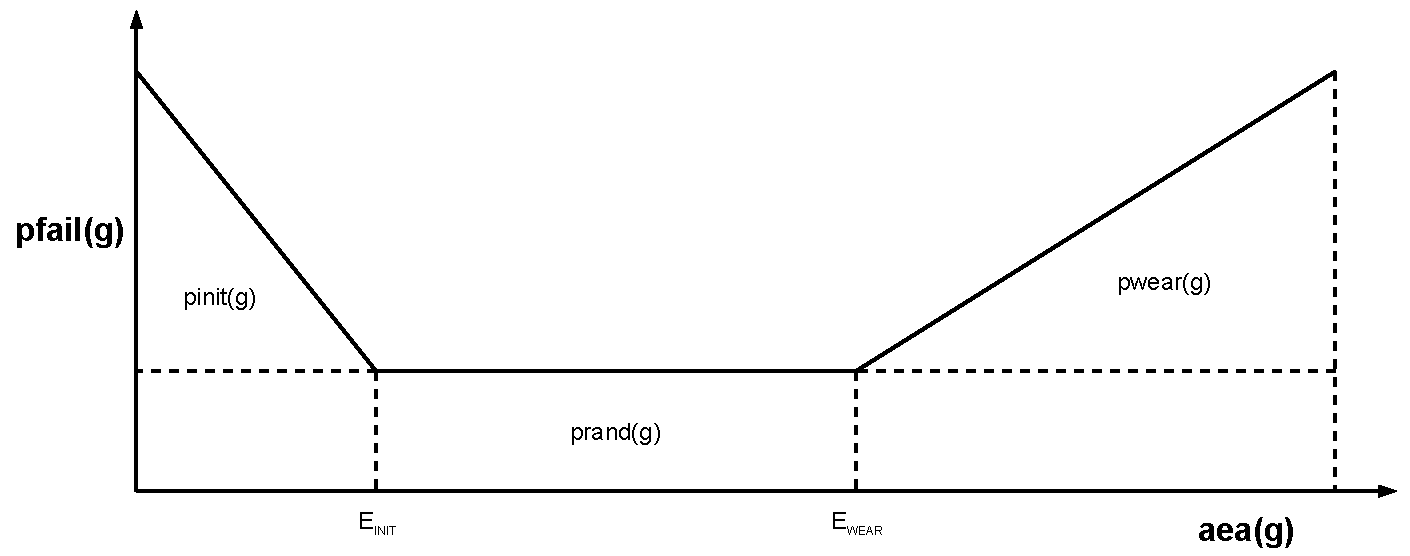
\includegraphics[width=0.7\linewidth]{node_reliability_lifespan}
	\caption[Probability of failure with lifetime energy usage for a node]{Probability of failure with lifetime energy usage for a node}
	\label{fig:node_reliability_lifespan}
\end{figure}
\begin{enumerate}
	\item $\functionProbabilityInit{}{}$, the initial failure probability, component failures early in lifespan, decreasing with time.
	\item $\functionProbabilityRand{}{}$, the random failure probability, the constant background failure rate.
	\item $\functionProbabilityWear{}{}$, the wear-out failure probability, the increasing failure rate towards the end of a nodes expected lifespan.
\end{enumerate}
For each node, we use $\functionAgentEnergyTotal{}{}$ as a proxy for time so the probability of an agent $\varAgent{}{}$ having a permanent failure increases with usage.

\definition[Probability of node failure]{
	The probability of node failure for an agent $\varAgent{}{}$ is $\functionProbabilityFail{}{}$, the combination of the probabilities of initial, random, and wear-out failures given the agents total energy usage in its lifetime $\functionAgentEnergyTotal{}{}$.
	\begin{equation}
		\functionProbabilityFail{}{} = \underbrace{max(0, (1 - \functionAgentEnergyTotal{}{}/\varEnergyInit{}{})) \times \varConstantInit{}{}}_{\functionProbabilityInit{}{}} + \underbrace{\varConstantRand{}{}}_{\functionProbabilityRand{}{}} + \underbrace{max(0, ( \functionAgentEnergyTotal{}{}/\varEnergyWear{}{}))\times \varConstantWear{}{}}_{\functionProbabilityWear{}{}}
	\end{equation}
	Where $\varEnergyInit{}{}{}{}$ is the energy level where initial failures are effectively zero,  and $\varEnergyWear{}{}{}{}$ where wear-out failures become a factor. $\varConstantInit{}{}$, $\varConstantRand{}{}$, and $\varConstantWear{}{}$  are constants chosen to scale the effects of initial failures and wear-out failures respectively.
}



